\section{Mô hình kiến trúc ứng dụng iOS}
Lựa chọn mô hình kiến trúc phù hợp là quyết định quan trọng ảnh hưởng đến khả năng bảo trì, mở rộng và kiểm thử của ứng dụng. Dưới đây là các mô hình phổ biến trong phát triển iOS:
Việc lựa chọn mô hình nào phụ thuộc vào nhiều yếu tố như quy mô dự án, kinh nghiệm nhóm phát triển và yêu cầu kỹ thuật cụ thể. Trong thực tiễn, lập trình viên iOS thường linh hoạt áp dụng kết hợp nhiều mô hình để tối ưu hóa khả năng mở rộng và dễ dàng kiểm soát sự phức tạp của ứng dụng.

\begin{figure}[H] 
    \centering
    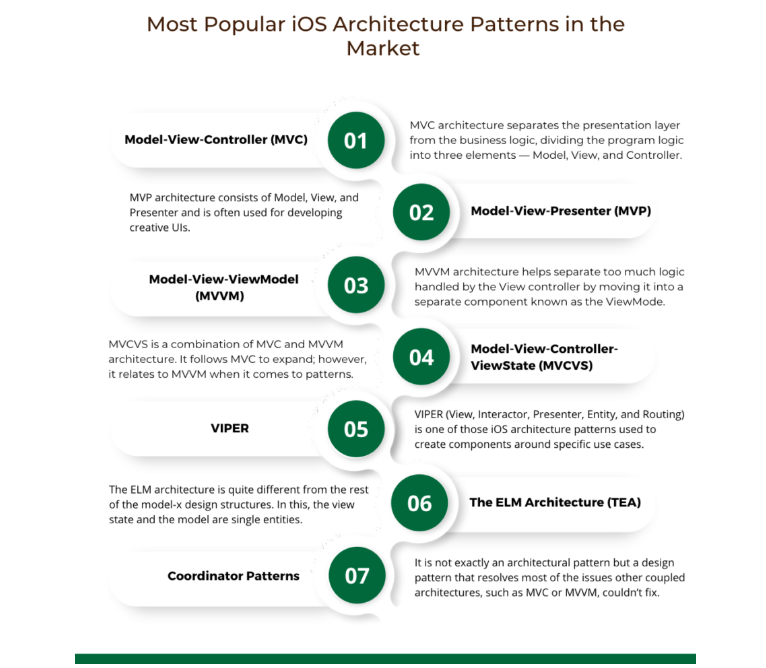
\includegraphics[width=0.8\textwidth]{images/mohinhkientrucios.png}
     \caption{Một số mô hình kiến trúc IOS}
    \label{fig:mohinhkientrucios}
\end{figure}
\subsection{Model–View–Controller (MVC)}
  Model–View–Controller (MVC) là một trong những mô hình kiến trúc truyền thống được Apple khuyến nghị sử dụng trong phát triển ứng dụng iOS. Mô hình này chia ứng dụng thành ba thành phần chính với vai trò rõ ràng nhằm tăng tính tổ chức và khả năng bảo trì mã nguồn.
  Thành phần đầu tiên, \textbf{Model}, là nơi quản lý dữ liệu và xử lý logic nghiệp vụ. Tiếp theo, \textbf{View} đảm nhiệm việc hiển thị giao diện người dùng và phản hồi các tương tác từ người dùng. Cuối cùng, \textbf{Controller} đóng vai trò trung gian, liên kết giữa Model và View, đồng thời xử lý các logic điều khiển và điều phối luồng dữ liệu.

  Một số ưu điểm nổi bật của mô hình MVC có thể kể đến như: đây là một mẫu kiến trúc phổ biến, không chỉ trong phát triển ứng dụng iOS mà còn cả trong phát triển web; nó cho phép phân tách rõ ràng trách nhiệm giữa các thành phần, đặc biệt là giữa phía máy chủ và máy khách; và nó rất phù hợp với các ứng dụng nhỏ, đơn giản nhờ tính dễ triển khai.

  Tuy nhiên, đi kèm với những lợi ích đó, MVC cũng tồn tại một số hạn chế. Nhược điểm lớn nhất là tình trạng \textit{"Massive View Controller"}, trong đó Controller trở nên quá lớn và phức tạp khi ứng dụng phát triển. Điều này không chỉ làm giảm khả năng kiểm thử mà còn khiến việc bảo trì trở nên khó khăn hơn do sự phụ thuộc chặt chẽ giữa các thành phần trong kiến trúc.

\subsection{Mô hình MVP trong iOS}

  Model-View-Presenter (MVP) là một biến thể của mô hình MVC, với mục đích tách biệt rõ ràng hơn giữa phần hiển thị (View) và logic điều khiển (Presenter). Sự phân tách này giúp tăng khả năng kiểm thử và tái sử dụng mã nguồn, đồng thời nâng cao tính linh hoạt trong việc thay đổi và mở rộng ứng dụng. 

  Thành phần của mô hình MVP gồm ba phần chính: \textbf{Model}, giống như trong mô hình MVC, quản lý dữ liệu và xử lý các logic nghiệp vụ; \textbf{View} là giao diện thụ động, chỉ có nhiệm vụ hiển thị dữ liệu và không tham gia vào việc xử lý logic; \textbf{Presenter} là thành phần xử lý toàn bộ logic nghiệp vụ và đảm nhận vai trò cập nhật dữ liệu cho View.

  Một số ưu điểm của mô hình MVP là: \textit{View} hoàn toàn thụ động, dễ dàng kiểm thử và duy trì; việc xác minh chức năng chính xác của từng thành phần trở nên dễ dàng hơn khi chúng được phân tách rõ ràng; \textit{Presenter} có thể được tái sử dụng với nhiều \textit{View} khác nhau, làm cho mã nguồn trở nên linh hoạt và dễ bảo trì.

  Tuy nhiên, mô hình MVP cũng có một số nhược điểm, bao gồm: sự cần thiết phải viết mã \textit{boilerplate} nhiều; \textit{Presenter} có thể trở nên quá lớn và phức tạp khi ứng dụng phát triển; và cuối cùng, MVP không phổ biến bằng mô hình MVVM trong cộng đồng iOS, làm cho việc tìm kiếm tài liệu và hỗ trợ trở nên khó khăn hơn.

\subsection{Mô hình MVVM trong iOS}

  MVVM (Model-View-ViewModel) là một mô hình kiến trúc hiện đại được áp dụng rộng rãi trong phát triển ứng dụng iOS, đặc biệt khi kết hợp với các framework reactive như Combine hoặc RxSwift. Mô hình này giúp tách biệt rõ ràng giữa giao diện người dùng và logic nghiệp vụ, tăng khả năng kiểm thử và dễ bảo trì.

  Mô hình MVVM bao gồm ba thành phần chính: \textbf{Model}, giống như trong các mô hình khác, có nhiệm vụ quản lý dữ liệu và logic nghiệp vụ; \textbf{View}, bao gồm các đối tượng \textbf{UIView} và \textbf{UIViewController}, chịu trách nhiệm hiển thị giao diện người dùng; và \textbf{ViewModel}, thành phần chịu trách nhiệm chuẩn bị dữ liệu từ Model và xử lý logic cần thiết để View có thể hiển thị dữ liệu.

  MVVM có bốn nguyên tắc quan trọng cần tuân thủ: \textbf{The Simplicity Principle} (Nguyên tắc đơn giản) yêu cầu mỗi View chỉ nên có một ViewModel và ngược lại; \textbf{The Blendability Principle} (Nguyên tắc hòa trộn) đề xuất ViewModel cần hỗ trợ tối ưu hóa UI; \textbf{The Designability Principle} (Nguyên tắc thiết kế) nhấn mạnh ViewModel phải cung cấp dữ liệu có thể sử dụng tại thời điểm thiết kế; và \textbf{The Testability Principle} (Nguyên tắc kiểm thử) yêu cầu cả Model và ViewModel phải có khả năng kiểm thử độc lập.

  Ưu điểm của mô hình MVVM bao gồm việc tách biệt rõ ràng các thành phần, dễ dàng kiểm thử (đặc biệt là ViewModel), giảm kích thước và trách nhiệm của ViewController, và hỗ trợ binding dữ liệu giữa View và ViewModel. Tuy nhiên, mô hình này cũng có một số nhược điểm, chẳng hạn như sự phức tạp hơn so với MVC, khả năng dẫn đến "Massive ViewModel" nếu không được tổ chức tốt, và yêu cầu cơ chế binding (thủ công hoặc sử dụng thư viện reactive).

  \subsection{MVCVS (Model-View-Controller-ViewState)}

  MVCVS là một sự kết hợp giữa hai kiến trúc MVC và MVVM, giúp tách biệt rõ ràng giữa \textbf{Model}, \textbf{View}, \textbf{Controller}, và \textbf{View State}. Trong mô hình này, \textbf{View State} giữ vai trò quan trọng trong việc theo dõi và cập nhật trạng thái giao diện người dùng.

  Ở giai đoạn \textbf{MVCVS Initialization}, View Controller phải tuân theo Model và View State để khởi tạo các thành phần. Khi có bất kỳ thay đổi nào trong \textbf{Model}, \textbf{MVCVS Model Updates} sẽ cập nhật Document Model và View State. Tiếp theo, trong giai đoạn \textbf{MVCVS View Changes}, View State sẽ phân tích Document View Model và View State, từ đó thực hiện các thay đổi đối với View dựa trên các quan sát. \textbf{MVCVS View State} tách biệt View Controller và View State, nơi View State chịu trách nhiệm cập nhật và lắng nghe các thay đổi trong View. Cuối cùng, \textbf{MVCVS Testability} cho phép kiểm tra logic của View Model và Document Model một cách riêng biệt, giúp việc kiểm thử hiệu quả hơn so với mô hình MVC.

  Về ưu điểm, MVCVS mang lại khả năng quản lý hiệu quả cao và dễ dàng kiểm tra các thành phần riêng biệt nhờ các bài kiểm tra tích hợp. Tuy nhiên, nó cũng có nhược điểm là độ phức tạp cao và khó tiếp cận đối với người mới.

  \subsection{VIPER}

  VIPER là một mẫu kiến trúc sạch, được sử dụng khi cần tạo các thành phần xoay quanh các trường hợp sử dụng cụ thể trong iOS. VIPER gồm năm thành phần chính: \textbf{View} (giao diện người dùng), \textbf{Interactor} (logic nghiệp vụ), \textbf{Presenter} (điều phối giữa View và Interactor), \textbf{Entity} (mô hình dữ liệu), và \textbf{Routing} (điều hướng giữa các màn hình).

  Ưu điểm của VIPER là dễ quản lý, đặc biệt khi làm việc với nhóm phát triển lớn. Nó giúp tăng khả năng tái sử dụng mã nguồn, kiểm soát UI và giúp dễ dàng kiểm thử mã nhờ vào việc phân tách các thành phần. Hơn nữa, nó giúp giảm thiểu xung đột hợp nhất mã. Tuy nhiên, VIPER có cấu trúc phức tạp đối với ứng dụng nhỏ, yêu cầu thời gian để làm quen và nhiều lớp trung gian có thể ảnh hưởng đến hiệu suất.

  \subsection{The Elm Architecture (TEA)}

  TEA là một mô hình kiến trúc đặc biệt trong iOS, khác biệt so với các cấu trúc Model-X truyền thống. Trạng thái giao diện và mô hình được hợp nhất thành một thực thể duy nhất, và mọi cập nhật được gửi đến thực thể này dưới dạng \textbf{messages} và xử lý thông qua \textbf{reducers}. Dòng sự kiện trong TEA được duy trì theo nguyên lý một chiều (unidirectional), tương tự như Flux hoặc Redux.

  Ưu điểm của TEA là khả năng mô tả View như các hàm thuần túy (pure functions) và thực hiện one-way binding từ Model đến View giúp dễ kiểm soát. Tuy nhiên, TEA cũng có nhược điểm, đó là nó tăng độ phức tạp trong các ứng dụng lớn và không phù hợp với mọi loại ứng dụng.

  \subsection{Coordinator Pattern}

  Coordinator không phải là một mẫu kiến trúc chính thức mà là một \textbf{design pattern}, giúp giải quyết các vấn đề điều hướng mà MVC hoặc MVVM không xử lý tốt. Coordinator chịu trách nhiệm tạo và giữ tham chiếu đến ViewController hiện tại, đồng thời thực hiện việc điều hướng giữa các màn hình, như việc hiển thị màn hình mới hoặc đẩy ViewController vào Navigation Controller.

  Một trong những ưu điểm lớn của Coordinator là khả năng tách riêng logic điều hướng, giúp mã dễ bảo trì và tăng tính linh hoạt khi chuyển đổi giữa các màn hình. Tuy nhiên, khi triển khai Coordinator, có thể làm tăng độ phức tạp của ứng dụng, yêu cầu thay đổi cách tiếp cận luồng dữ liệu và không cần thiết cho các ứng dụng nhỏ.